
\subsection{System Architecture}
\label{subsec:methodology-system-overview}

GaitNet is the high-level footstep planner in a hierarchical
locomotion stack. At each control tick, the robot receives a terrain
height scan. The scan is converted into steppable and unsteppable
cells. The mask is dilated to account for foot size and
state-estimation error. It is then converted into a per-leg validity
mask. \changed{GaitNet scores every valid cell in that mask. It
compares those footstep candidates with a learned no-action option.
It then sends the best single action to the low-level tracking
controller.} The action contains one leg, one target foothold, and one
swing duration.

The tracking layer depends on the platform. In simulation, GaitNet
runs through the MIT Mini-Cheetah Controller
\cite{di_mini_cheetah_2020}. We use the Python structure from
\cite{zhuang_rl_mpc_locomotion_2025}. On hardware, the same GaitNet
action replaces the native gait scheduler in the Legged Perceptive
Stack. The stack then tracks the action with its NMPC/Whole-Body
Control (WBC) pipeline \cite{leggedperceptive}. This separation makes
the hardware comparison focus on the planner. The low-level
controller stays fixed. \changed{Using a frozen learned planner with a
different model-based execution layer is also consistent with prior
policy retargeting results \cite{li_zero-shot_2022}.}

Two feasibility rules run before the network scores a candidate.
First, a leg that is already swinging is removed from the mask. Its
target is not redirected in mid-swing. Second, a new step is allowed
only if at least \numberstringnum{\corlMinContactLegs} legs remain in
ground contact. This limits concurrency to
\numberstringnum{\corlMaxConcurrentSwingLegs} swing legs. We use this
explicit stability constraint in every experiment in
\autoref{sec:results}. The terrain mask is also dilated with
\numberstringnum{\corlMaskDilationRounds} rounds of max pooling. This
treats small gaps near a candidate foothold edge conservatively.

\begin{figure*}[t]
  \centering
  % Source of truth is images/diagrams/gaitnet-architecture.svg (edit in
  % Inkscape). The PDF beside it is exported from that SVG for pdflatex:
  %   inkscape --export-type=pdf gaitnet-architecture.svg
  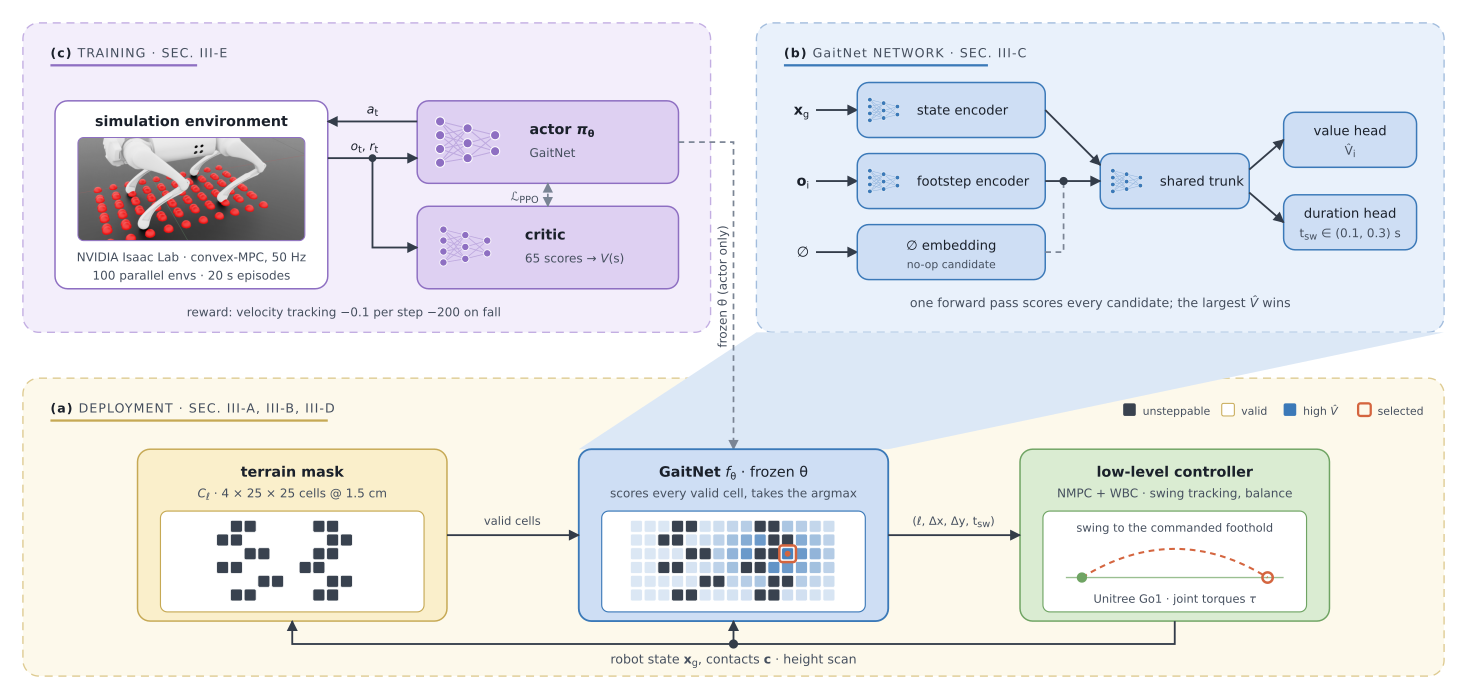
\includegraphics[width=\textwidth]{ICRA/images/diagrams/gaitnet-architecture.png}
  \caption{\changed{System overview. (a)~Deployment: a height scan
    becomes a per-leg validity mask; GaitNet scores every valid cell
    plus a no-action option in one pass, and the argmax is issued as a
    single footstep command. (b)~The network: state and candidate
    embeddings feed a shared trunk with value and duration heads.
    (c)~Training: PPO in Isaac Lab over a sampled 65-candidate set;
    only the actor is deployed, frozen.}}
  \label{fig:diagram-control-system}
\end{figure*}

\subsection{High-Rate Action Selection}
\label{subsec:methodology-high-rate-selection}

GaitNet runs at \corlControlHz\,Hz, or once every
\corlControlTickMs\,ms. Each tick can issue at most one footstep for
one leg. All other legs keep their current commands. A selected swing
lasts between \corlSwingDurationMin\,s and
\corlSwingDurationMax\,s. This means
\numberstringnum{\corlMinTicksPerSwing} to
\numberstringnum{\corlMaxTicksPerSwing} planner ticks occur before
that leg touches down. During those ticks, GaitNet may choose to
swing another leg. The only limit is the contact-count rule above.

This timing creates acyclic coordination. The planner never chooses a
gait phase, leg pair, or contact sequence. Instead, it repeatedly asks
a simple question: is any available footstep better than doing
nothing? If yes, and another leg is already in swing, the swings
overlap. If the no-action option wins, the robot waits.
\changed{Learned per-candidate scoring has already made acyclic
contact planning fast enough for online use
\cite{bratta_contactnet_2024, taouil_non-gaited_2024}. The
single-leg, single-tick action space used here makes the decision
small enough to repeat every control tick, not only at contact
events.}

\subsection{GaitNet Formulation}
\label{subsec:methodology-gaitnet-architecture}

GaitNet evaluates candidate actions with one neural network. The
network has a robot-state encoder, a footstep encoder, a shared trunk,
and two output heads. The value head outputs the unnormalized logit
$\hat{V}$ used to rank a candidate. The duration head predicts the
swing duration used if that candidate is selected.

Each candidate is conditioned on the current tracking state
$\mathbf{x_g}$ and a one-hot action identity that represents either a
leg-specific foothold or the no-action option:
\begin{equation}
  \mathbf{x_g} =
  \begin{bmatrix}
    \mathbf p_{f,xy}^{b} &
    p_{b,z} &
    \mathbf v_b &
    \mathbf \omega_b &
    \mathbf v^{usr} &
    \mathbf c &
    \mathbf g_b
  \end{bmatrix}^T .
  \label{eq:gaitnet-x}
\end{equation}
Here $\mathbf p_{f,xy}^{b} \in \mathbb{R}^{\corlFootPosDim}$ contains
the $xy$ positions of all four feet in the base frame. The scalar
$p_{b,z}$ is the base height in the world frame. The vectors
$\mathbf v_b \in \mathbb{R}^{\corlVelDim}$ and
$\mathbf \omega_b \in \mathbb{R}^{\corlAngVelDim}$ are the linear and
angular velocity in the root frame. The commanded velocity is
$\mathbf v^{usr} = [v_x, v_y, \omega_z]$. The contact state is
$\mathbf c \in \{0,1\}^{\corlContactDim}$. The vector
$\mathbf g_b \in \mathbb{R}^{\corlGravityDim}$ is projected gravity in
the body frame. The full state has \corlStateDim{} dimensions. Unlike
ContactNet \cite{bratta_contactnet_2024}, this formulation includes
angular velocity. This gives the value function direct access to body
rotation.

The network uses a middle-fusion feature structure \cite{feng2021deep}:
\begin{itemize}
  \item \textbf{Robot state encoder:} a
    \numberstringnum{\corlStateEncoderLayers}-layer Multi-Layer
    Perceptron (MLP) maps the \corlStateDim-dimensional tracking state
    to a latent state representation using hidden dimension
    \corlStateEncoderHidden{} and ReLU activations.
  \item \textbf{Footstep encoder:} a
    \numberstringnum{\corlFootstepEncoderLayers}-layer feedforward
    network embeds each candidate's leg identity and spatial offset
    using hidden dimension \corlFootstepEncoderHidden{} and ReLU
    activations. The no-action option has no spatial offset and uses a
    separate learned embedding.
  \item \textbf{Shared trunk:} the state and candidate embeddings are
    concatenated and passed through a
    \numberstringnum{\corlTrunkLayers}-layer MLP with ReLU
    activations.
  \item \textbf{Output heads:} the value head outputs $\hat{V}$, while
    the duration head outputs $t_{\text{swing}}$, scaled by a sigmoid
    into $(\corlSwingDurationMin, \corlSwingDurationMax)$\,s.
\end{itemize}

The evaluated configuration does not use a separate learned cost
input. Our preliminary framework \cite{Sullivan2025} included a
footstep-evaluation network. It scored candidates before GaitNet
ranked them. An ablation showed that zeroing this cost input improved
survival rate. We therefore remove that stage. GaitNet's value head is
the only ranking signal.

\begin{changedblock}
\subsection{Candidate Enumeration and Selection}
\label{subsec:methodology-gaitnet-selection}

At deployment, GaitNet does not sample candidate footholds. Each leg's
mask is a $\corlGridCells \times \corlGridCells$ grid at
\corlMaskResolutionCm\,cm resolution. The grid is centered on the
corresponding hip and spans $\pm\corlGridReachCm$\,cm. Across four
legs, this gives $\corlNumLegs \times \corlCellsPerLeg =
\corlSpatialCandidates$ possible footholds. With the no-action option,
there are \corlTotalCandidatesDense{} total candidates.

Exhaustive scoring is efficient because the candidate embedding does
not depend on the robot state. The leg one-hot and spatial offset for
each grid cell are fixed. Their embeddings are computed once at
startup and cached. Each control tick then needs one state-encoder
pass and one batched shared-trunk pass over the candidate set. Scoring
all \corlTotalCandidatesDense{} candidates takes \corlDenseScoreMs\,ms
and matches an unfactored forward pass to within
$\corlDenseAgreement$. Invalid cells are removed by the mask before
scoring. A typical tick therefore evaluates fewer candidates than the
full grid.

This dense pass is faster and more reliable than deployment-time
sampling. Recreating the \corlTrainTotalCandidates{}-candidate sampled
set used during training takes \corlSampledScoreMs\,ms. Sampling can
also miss the highest-valued valid cell. GaitNet therefore selects the
exact argmax of $\hat{V}$ over all valid cells and the no-action
option. If no-action has the highest score, or no leg has a valid
cell, the planner issues no footstep on that tick.

The key property is independent candidate scoring. The number of
candidates is not built into the learned weights. The actor is trained
on \corlTrainTotalCandidates{} sampled candidates
(\autoref{subsec:methodology-gaitnet-training}). At deployment, it is
used frozen on up to \corlTotalCandidatesDense{} enumerated
candidates. No retraining or fine-tuning is used.
\end{changedblock}

\subsection{Reinforcement Learning Framework}
\label{subsec:methodology-gaitnet-training}

Stable labels for optimal footstep choices are hard to generate. The
value of a step depends on future contacts, body motion, and terrain
interactions. GaitNet is therefore trained with reinforcement learning
using Proximal Policy Optimization (PPO)
\cite{Schulman_proximal_2017}.

The actor is the GaitNet network described above. The critic is a
separate, smaller network. It has its own state encoder, footstep
encoder, and trunk. \begin{changedblock}For each sampled candidate,
the critic produces a score. A small combining MLP maps all
\corlTrainTotalCandidates{} candidate scores to one state-value
estimate. The critic shares no weights with the actor. It also has no
duration head.

Training uses a sampled candidate set. For each leg,
\numberstringnum{\corlTrainCandidatesPerLeg} candidates are drawn
uniformly from the valid terrain mask. One no-action option is added.
This gives \corlTrainTotalCandidates{} candidates per decision. The
actor's logits over this sampled set define a categorical
distribution. Training a scalar per-candidate score as an unnormalized
logit over an enumerated set is related in objective form to implicit
behavioral cloning \cite{florence_implicit_2021}. Here, however, the
policy is optimized with PPO rather than supervised labels.

The training and deployment candidate distributions differ on purpose.
Sampling keeps the categorical distribution and entropy term bounded
during training. The actor is still a per-candidate scorer, so it can
be evaluated on a denser set at deployment. The deployed grid is a
superset of the sampled training grid. Deployment changes how many
candidates are compared. It does not change the type of candidate the
network sees. This width-agnostic property applies only to the actor.
The critic's combining MLP is fixed to
\corlTrainTotalCandidates{} inputs and is discarded after training.
\end{changedblock}

For the selected candidate, the duration output defines the mean of a
Normal distribution. The distribution has fixed standard deviation
\corlDurationExploreStd\,s. The action log probability is the sum of
two terms: the categorical log probability of the selected candidate
and the Normal log probability of the sampled duration. Rewards
balance velocity tracking, stability, and a small per-step action
penalty ($\corlActionPenalty$). This penalty discourages unnecessary
steps. Falling or stepping onto invalid terrain triggers termination
with a $\corlTerminationPenalty$ penalty. Reward tables, termination
conditions, command ranges, and PPO hyperparameters follow
\cite{Sullivan2025}.

Training is performed in NVIDIA Isaac Lab \cite{mittal_orbit_2023}.
Physics and policy inference run on the GPU. The MPC controllers run
in parallel on the CPU across \corlParallelEnvs{} simulated
environments. The model is trained for \corlTrainingIterations{}
iterations. A terrain curriculum gradually increases the fraction of
unsteppable cells \cite{Sullivan2025}.
